\section{Surface Acoustic Waves and how they can be created}

True to their name, \emph{Surface Acoustic Waves (SAW)} are sonic waves that propagate along the surface of a solid material. 
The expression is an umbrella term for several kinds of waves that fall under this description, but the type of waves that is relevant to the application researched in this thesis is called \emph{Rayleigh Waves} \cite{mandalSurfaceAcousticWave2022}.

Rayleigh waves are a superposition of a longitudinal (P) and a shear vertical (SV) wave component and propagate through the surface of the substrate, with the amplitude of the particle motion decreasing exponentially along the depth of the material. 
Typically, the effective penetration in the direction normal to the surface is less than a wavelength. 
Because of how these longitudinal and vertical components the waves produce an elliptical motion in the surface particles, with the plane of the ellipsis being parallel to the direction of propagation and normal to the material surface (see Figure \ref{fig:rayleigh}).

\begin{figure}[htbp]
    \centering
    \makebox[\textwidth][c]{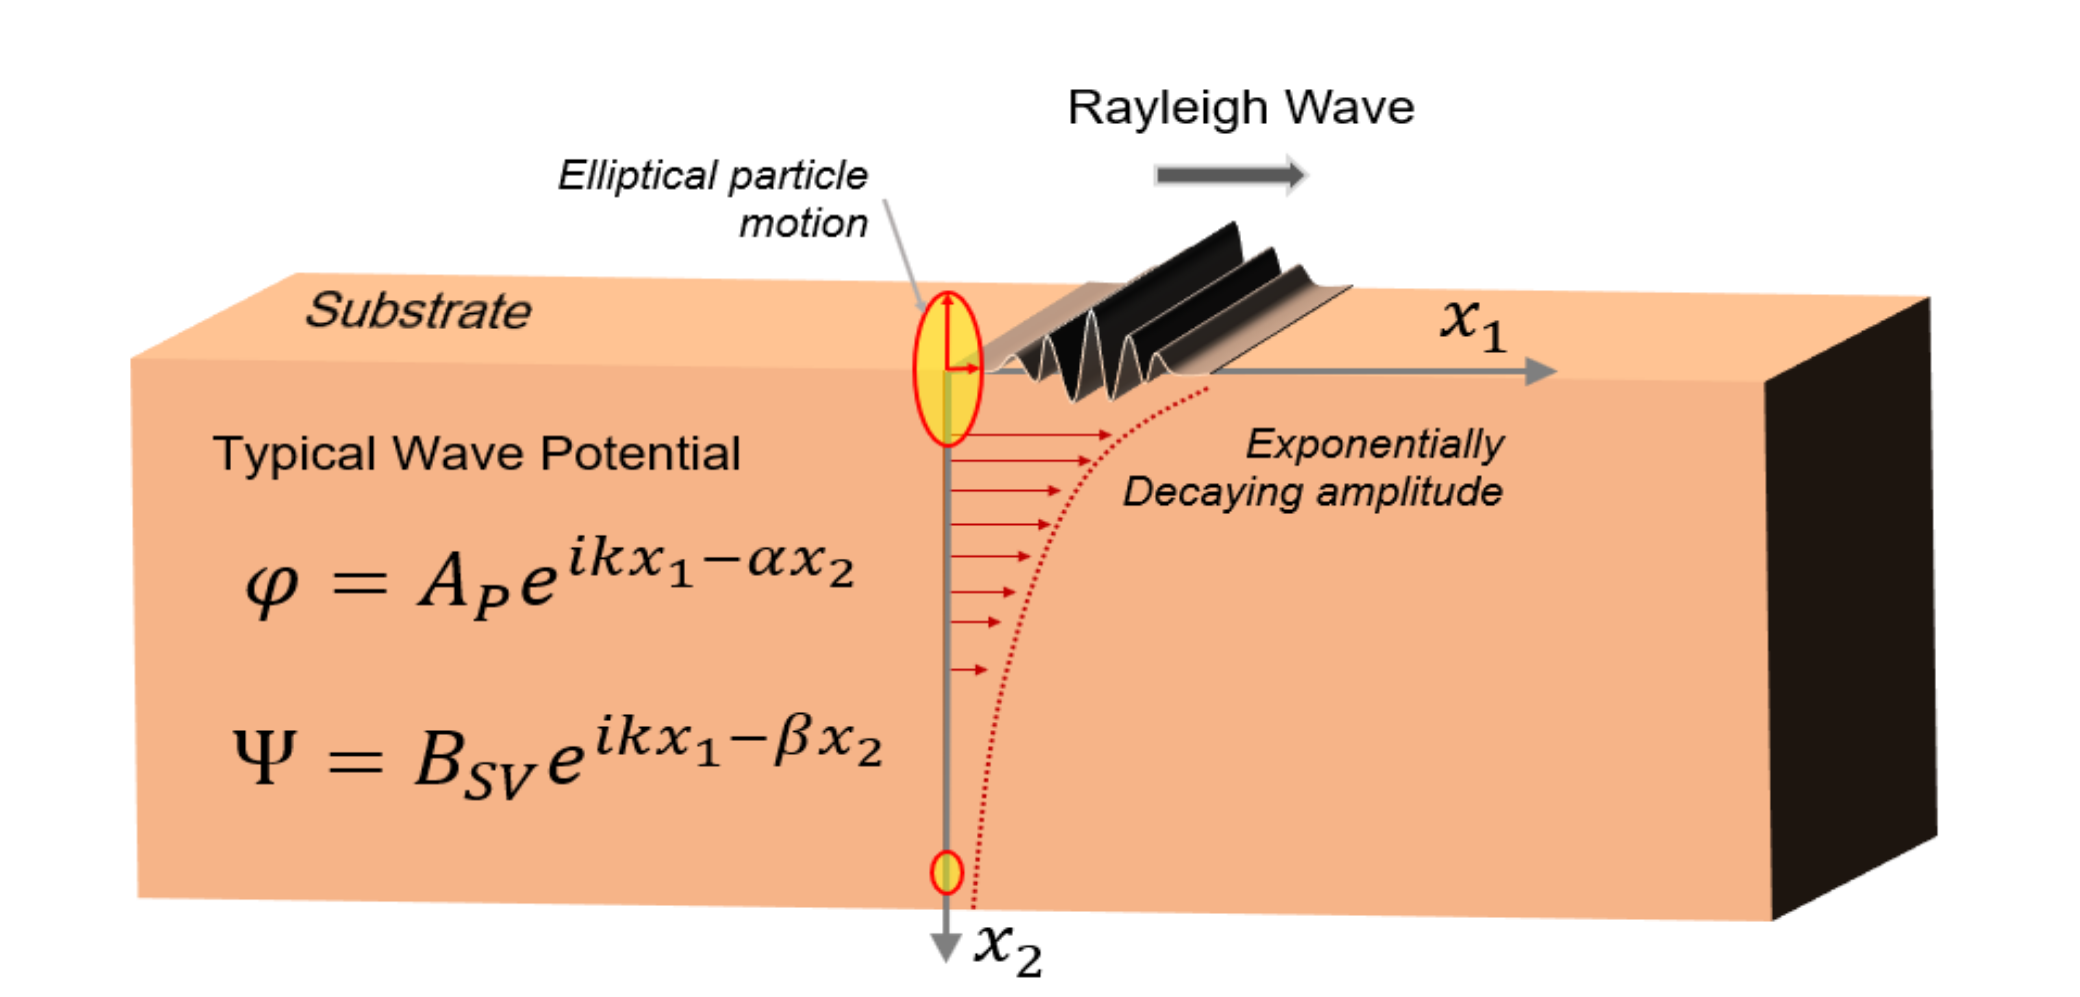
\includegraphics[width=0.8\textwidth]{images/Screenshot-20230208172733-2080x997.png}}
    \caption{Depiction of Rayleigh-Waves propagating through a substrate. \cite{mandalSurfaceAcousticWave2022}}
    \label{fig:rayleigh}
\end{figure}

Other types of SAW waves include \emph{Shear Horizontal Waves} and \emph{Lamb Waves}, however these wave types do not cause the strong vertical displacement which is of interest for the purpose of liquid atomization. From now on the term SAW will be used synonymously for Rayleigh Waves.

For most applications, SAW are produced by fixing an \emph{interdigital transducer} (IDT) to a \emph{piezoelectric} substrate. An IDT is a type of electrode structure consisting of two sets of interleaved metal fingers, which are connected to the opposite poles of a radio frequency signal source. Applying an RF voltage to the IDT produces surface waves by exploiting the piezoelectric properties of the substrate.

A piezoelectric material generates an electrical voltage in response to applied mechanical stress, and conversely generates mechanical displacement in response to applied electrical voltage. 
The piezoelectric effect stems from the relative displacement of oppositely charged ions in a crystal with asymmetrical unit cells causing a displacement of the charge concentration and resulting in a larger electric dipole moment. 
If the dipoles in the crystal are aligned, the effect causes the whole crystal to be polarized, creating an electric voltage. 
Since the dipole moments in a crystal are typically only aligned locally in their respective Weiss domains, materials usually need to be poled in order to exhibit strong piezoelectric properties \cite{liLeadfreePiezoelectricMaterials2021}.
All piezoelectric materials also exhibit the reverse effect; applying an electrical field exerts electrostatic force on the dipoles which causes displacement of the ions.

\begin{figure}[htbp]
    \centering
    \makebox[\textwidth][c]{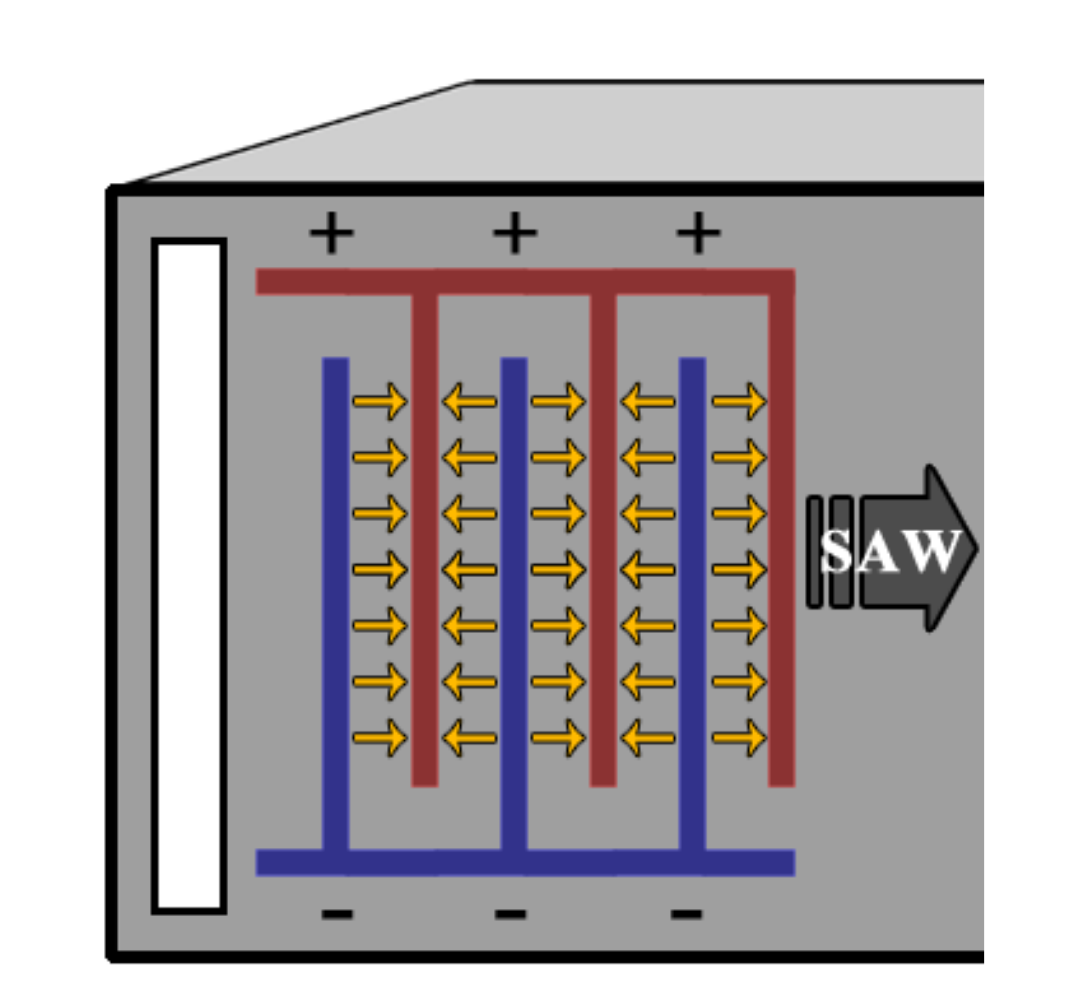
\includegraphics[width=0.4\textwidth]{images/Screenshot-20230208192523-1078x984.png}}
    \caption{The principle of SAW generation in a piezoelectric substrate. A voltage is applied to the two parts of an IDT, which causes mechanical tension in the substrate.}
    \label{fig:idt}
\end{figure}

Since the mechanical force caused by the phenomenon is parallel to the electrical field, applying high frequency voltage to the electrodes arranged in this interwoven pattern (see Figure \ref{fig:idt}) generates surface waves perpendicular to the direction of the electrodes.

The wavelength of the SAW is determined by the distance between the electrodes, which allows for a fine control of the wave frequency for each particular device.

Conversely, the same construction can be used to to pick up vibrations and convert them back to electrical voltage. 
This is the principle commonly used in SAW based sensors, which is only one of many useful applications of SAW technology like filtering in radio frequency technology or compact voltage transformers. 
In the next section the possible application for fluid atomization will be further discussed.